\documentclass[conference]{IEEEtran}

\ifCLASSINFOpdf

\else
  \usepackage[dvipdfmx]{graphicx}
  \usepackage{subfig}
\fi

\hyphenation{op-tical net-works semi-conduc-tor}


\begin{document}

\title{Write your paper title}

\author{\IEEEauthorblockN{Daiki Hiraoka\textsuperscript{1},
Shin-ichi Ito\textsuperscript{2},
Momoyo Ito\textsuperscript{3} and
Minoru Fukumi\textsuperscript{4}}
  \IEEEauthorblockA{Tokushima University, 2-1 Minami-Josanjima, Tokushima, 770-8506 Japan}
  \IEEEauthorblockA{\textsuperscript{1}c501537004@tokushima-u.ac.jp,\textsuperscript{2}s.ito@tokushima-u.ac.jp,\textsuperscript{3}momoito@is.tokushima-u.ac.jp,\textsuperscript{4}fukumi@is.tokushima-u.ac.jp}
}


\maketitle


\begin{abstract}
This section is abstract.
You write abstract of your study.

\end{abstract}


\IEEEpeerreviewmaketitle


\section{Introduction}
  This section is introduction.
  If you want to use image, you should write below.\figurename \ref{fig:gaussian_function}.

  \begin{figure}[!t]
    \centering
    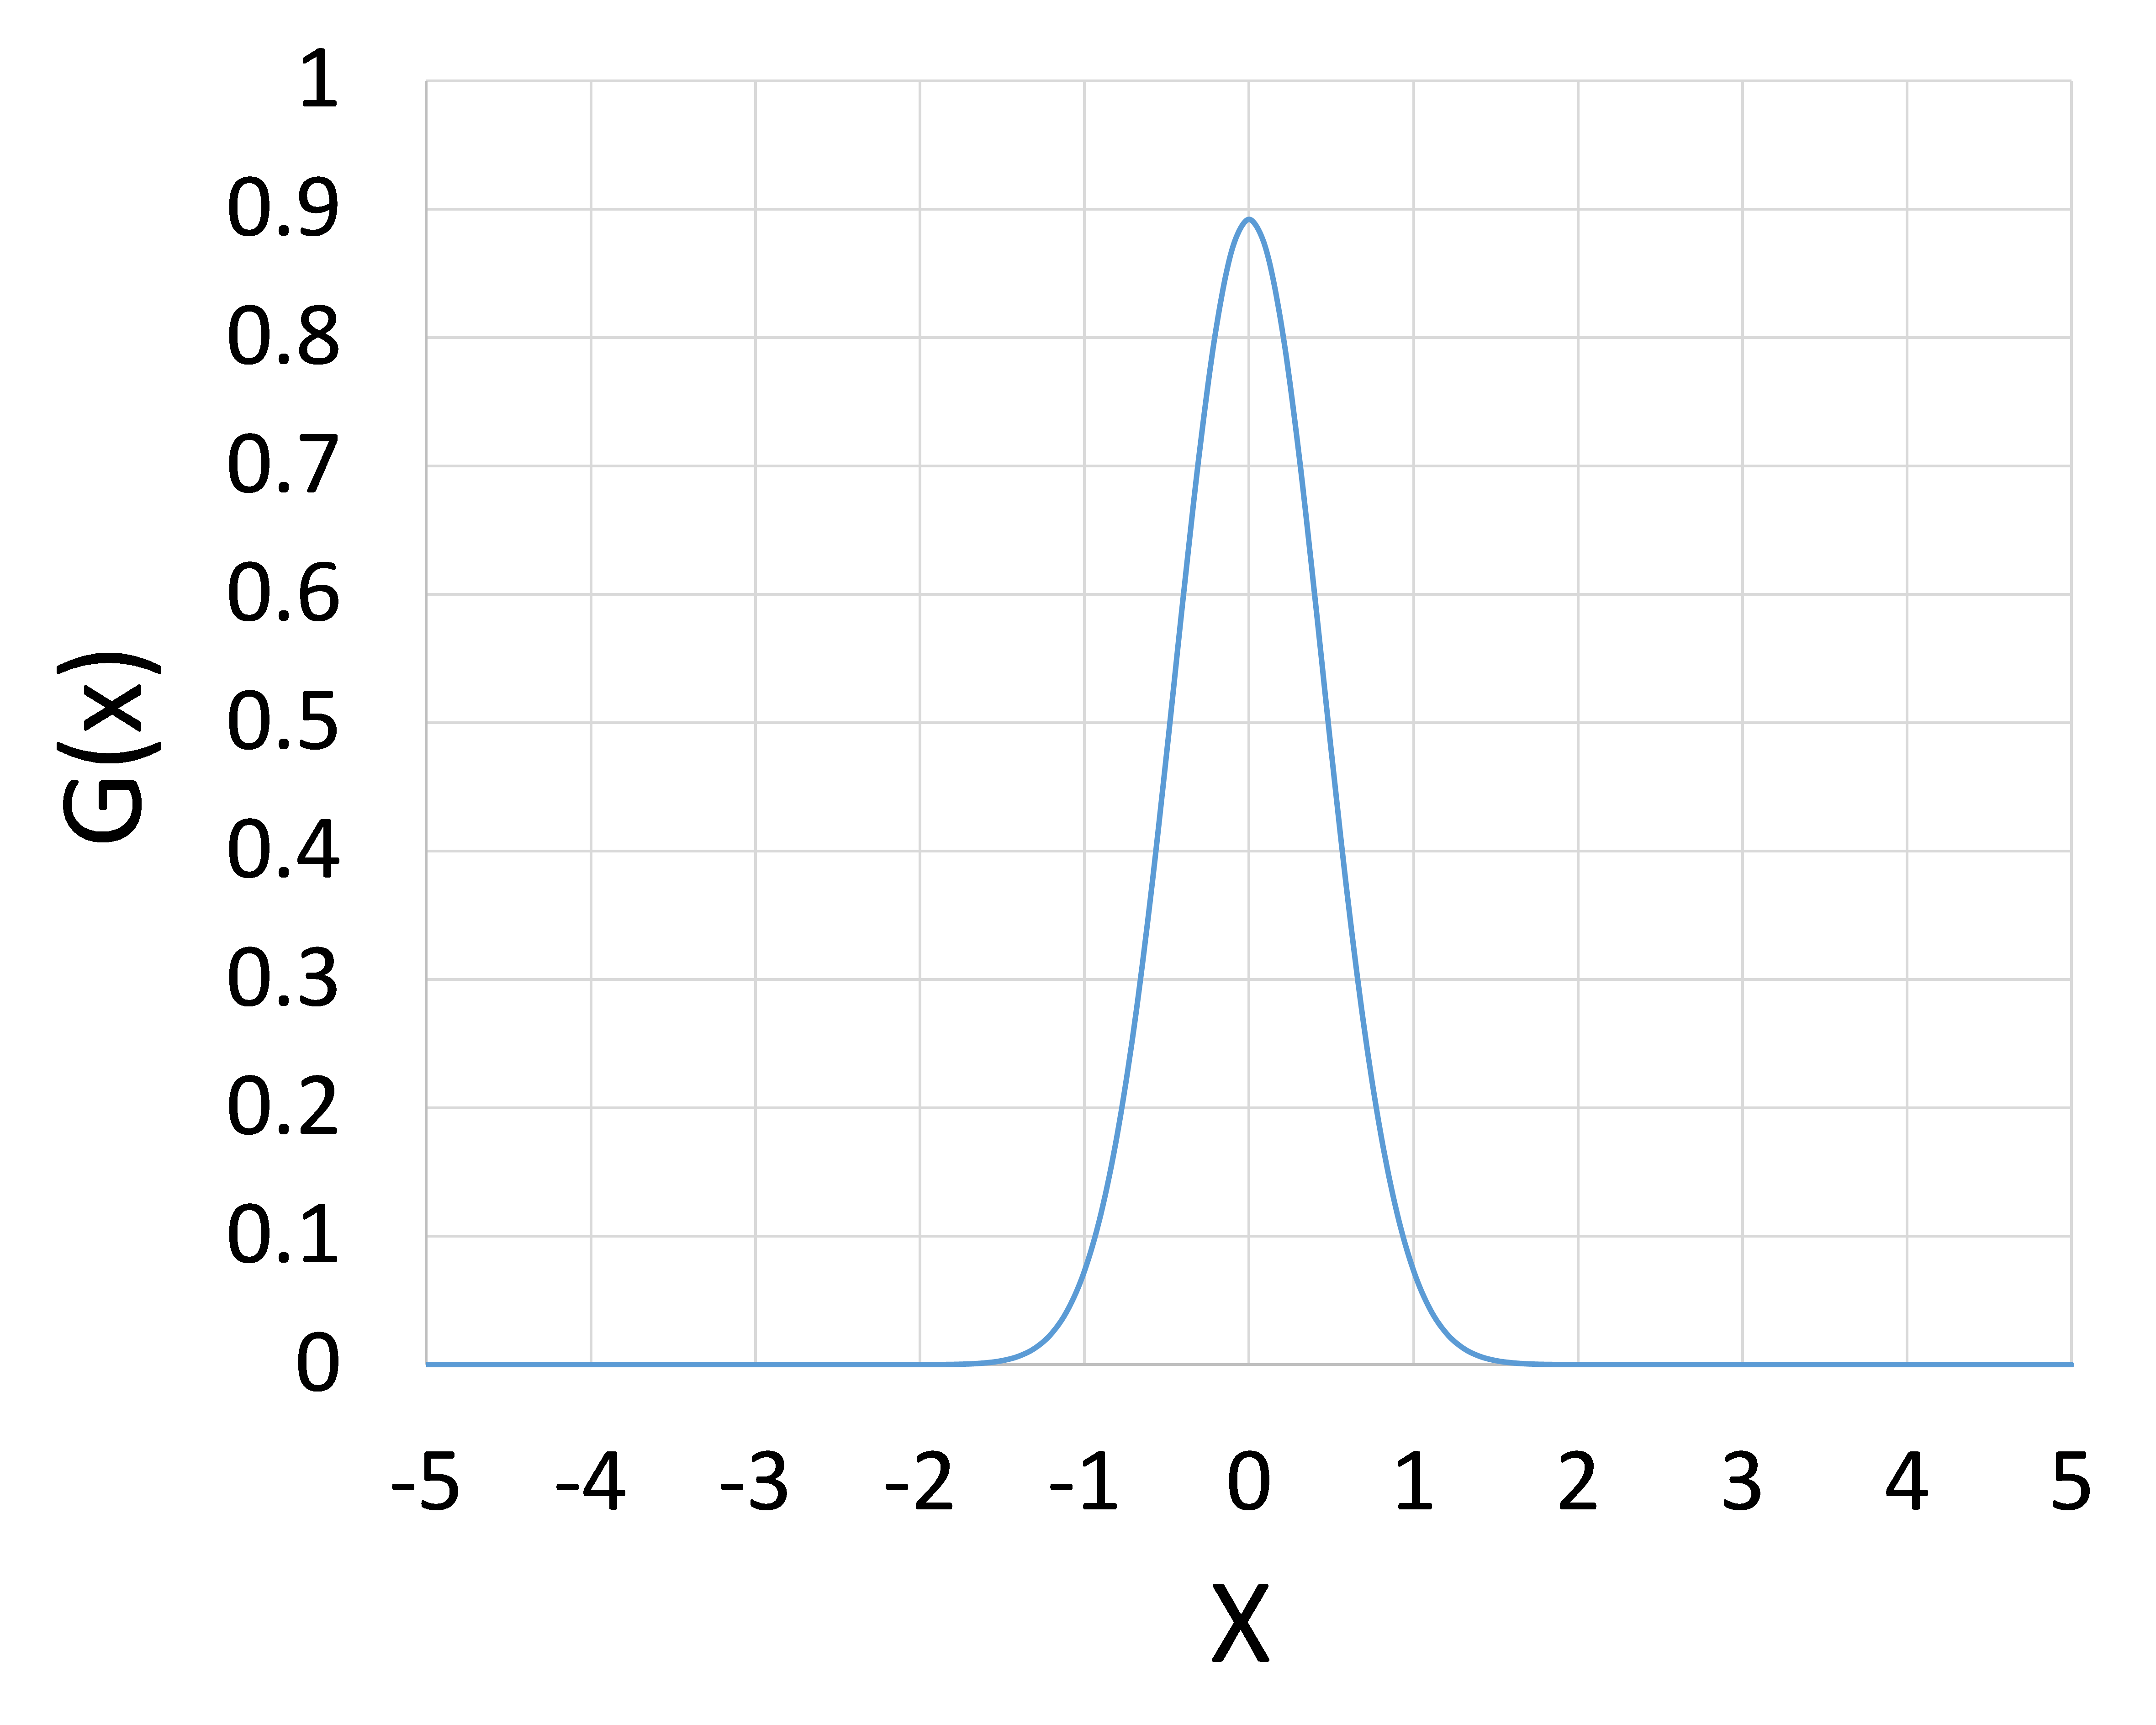
\includegraphics[width=2.5in]{./images/gaussian_function.png}
    \caption{Motions of Japanese Janken}
    \label{fig:gaussian_function}
  \end{figure}

  This is eqnarray sample.

  \begin{eqnarray}
    tn & = & \frac{y_{neutral1} + y_{neutral2} + ... + y_{neutral10}}{10}\\
    tr & = & \frac{y_{rock1} + y_{rock2} + ... + y_{rock10}}{10}\\
    ts & = & \frac{y_{scissors1} + y_{scissors2} + ... + y_{scissors10}}{10}\\
    tp & = & \frac{y_{paper1} + y_{paper2} + ... + y_{paper10}}{10}
  \end{eqnarray}

  This is table sample.

  \begin{table}[!t]
    \renewcommand{\arraystretch}{1.3}
    \caption{Discrimination Accuracy of the Previous Method}
    \label{table:prev_method_result}
    \centering
    \begin{tabular}{c||c|c|c}
      \hline
      \bfseries Motion & \bfseries Subject A & \bfseries Subject B & \bfseries Subject C\\
      \hline\hline
      Neutral & 100.0 \% & 98.0 \% & 80.0 \%\\\hline
      Rock & 92.0 \% & 80.0 \% & 90.0 \%\\\hline
      Scissors & 64.0 \% & 2.0 \% & 4.0 \%\\\hline
      Paper & 92.0 \% & 96.0 \% & 100.0 \%\\\hline\hline
      All & 87.0 \% & 69.0 \% & 68.5 \%\\\hline
    \end{tabular}
  \end{table}

\section{Previous Method}
This section is Previous Method.


\section{Proposed method}
This section is Proposed method.

\section{Experiment}
  This section is Experiment.

  \subsection{Experimental Conditions}
    This subsection is Experimental Conditions

\section{Results and Consideration}
  This section is Results and Consideration.

\section{Conclusion}
  Last section of this paper.

\begin{thebibliography}{3}

\bibitem{SVM1}
Yanzhao Chen, Yiqi Zhou, Xiangli Cheng and Yongzhen Mi: Upper Limb Motion Recognition Based on Two-Step SVM Classification Method of Surface EMG, International Journal of Control and Automation, Vol.6, No.3, June, 2013.

\end{thebibliography}

\end{document}
